\documentclass[10pt,twocolumn,letterpaper]{article}

\usepackage[margin=0.75in]{geometry}
\usepackage{times}
\usepackage{microtype}
\usepackage{epsfig}
\usepackage{graphicx}
\usepackage{amsmath}
\usepackage{amssymb}
\usepackage{booktabs}
\usepackage{xcolor}
\usepackage{colortbl}
\usepackage{multirow}
\usepackage{subcaption}
\usepackage{cite}
\usepackage[pagebackref=true,breaklinks=true,letterpaper=true,colorlinks,bookmarks=false,citecolor=blue,linkcolor=blue,urlcolor=blue]{hyperref}

% Document Metadata
\title{\textbf{QuadTree-JEPA: Hierarchical Multi-Scale Self-Supervised Joint-Embedding Predictive Architecture for Fine-Grained Visual Representation}}

\author{
  \textbf{Prithvi S}$^{1}$ \\
  $^{1}$Independent Researcher \\
  \texttt{prithvi@project-quadtree.org}
}

\date{Preprint — September 2026}

\begin{document}

\maketitle

\begin{abstract}
Standard Vision Transformers (ViTs) discretize images into a uniform grid of fixed-size patches. In fine-grained visual domains, this creates a fundamental tension: coarse patches ($16\!\times\!16$) catastrophically dilute localized micro-structures (foliar lesions, plumage details), while fine-grained uniform patches explode sequence length quadratically. We propose \textbf{QuadTree-JEPA}, a hierarchical multi-scale self-supervised framework that couples adaptive quadtree spatial decomposition with a Joint-Embedding Predictive Architecture (JEPA). Our core contribution is a \textit{fully vectorized, deterministic-budget QuadTree tokenizer} that partitions images into a 4-level spatial pyramid (patch sizes $64\!\times\!64$ down to $8\!\times\!8$) under a strict $K\!=\!256$ token budget, eliminating all host-device PCIe synchronization stalls and enabling dense $(B, 256, D)$ Tensor Core batch collation. Tokens are mapped to a shared embedding dimension via a \textit{Multi-Scale Z-Axis Fusion Bridge} combining grouped GEMM projections, continuous 2D sinusoidal spatial encodings, and learnable 1D scale embeddings. A \textit{stochastic bidirectional cross-scale masking} policy trains the model to predict fine-scale representations from coarse context and vice versa, operating entirely in latent space to avoid pixel-level reconstruction artifacts. Evaluated on an 18-class Plant Pathology benchmark (25,283 images), QuadTree-JEPA achieves \textbf{90.65\% accuracy} and \textbf{88.22\% macro F1} after self-supervised pre-training and end-to-end fine-tuning. The label-efficiency benchmark infrastructure (comparing frozen JEPA linear probes against supervised ViT baselines of matched capacity) is implemented and awaits execution across label-scarce regimes.
\end{abstract}

\section{Introduction}
\label{sec:intro}

The Vision Transformer (ViT)~\cite{dosovitskiy2020image} processes images as a sequence of fixed-size non-overlapping patches. With pairwise self-attention complexity $\mathcal{O}(N^2)$ over token sequence length $N$, practitioners must choose patch sizes $P \ge 14$ to keep memory tractable. For fine-grained visual benchmarks—botanical leaf pathology, aviary species classification~\cite{wah2011caltech}—this uniformity creates a severe inductive mismatch: discriminative micro-structures (e.g., fungal sporulation patterns, feather barb microstructure) occupy a minority of image pixels, while large homogeneous regions (background soil, sky) dominate the token budget.

Classical quadtree patch decompositions~\cite{tang2022quadtree} address this by recursively subdividing high-variance spatial regions, but suffer from two systems-level bottlenecks that have prevented their use in large-scale self-supervised pre-training:

\begin{enumerate}
    \item \textbf{Non-deterministic token counts:} Adaptive recursion yields variable-length sequences per image, preventing dense $(B, N, D)$ batch collation and forcing serial per-image GPU inference ($B=1$).
    \item \textbf{Host-device synchronization:} Scalar `.item()` variance threshold comparisons require synchronizing GPU tensors to CPU on every recursive branching decision, stalling the GPU pipeline.
\end{enumerate}

We resolve both problems with a \textit{deterministic-budget vectorized} formulation that fixes exactly $K=256$ tokens per image regardless of image content, executed entirely on-device with zero CPU synchronization.

For the self-supervised learning objective, we build on the Joint-Embedding Predictive Architecture (I-JEPA)~\cite{assran2023self}, which learns representations by predicting target patch embeddings from context embeddings entirely in latent space—avoiding the pixel reconstruction artifacts~\cite{he2022masked} that arise when multi-scale tokens must decode high-frequency texture details. We extend JEPA with a stochastic bidirectional cross-scale masking strategy that forces the model to bridge hierarchical abstraction levels.

\textbf{Summary of contributions:}
\begin{itemize}
    \item A fully vectorized deterministic-budget QuadTree tokenizer that eliminates all CPU synchronization stalls and enables dense batch collation.
    \item A Multi-Scale Z-Axis Fusion Bridge with grouped GEMM projections and joint 2D spatial + 1D scale positional encodings.
    \item A stochastic bidirectional cross-scale JEPA masking policy (coarse$\to$fine and fine$\to$coarse prediction modes).
    \item A Scale-Aware Attentive Pooling head with zero-initialized learnable level biases for stable downstream classification.
    \item An empirically verified result of \textbf{90.65\% accuracy and 88.22\% macro F1} on an 18-class Plant Pathology benchmark with 25,283 images.
\end{itemize}

%-------------------------------------------------------------------------
\section{Related Work}
\label{sec:related}

\subsection{Vision Transformers \& Efficient Tokenization}
The original ViT~\cite{dosovitskiy2020image} demonstrated that pure attention over uniform patches scales competitively with CNNs on large datasets. Hierarchical architectures—Swin Transformer~\cite{liu2021swin} and Pyramid Vision Transformer~\cite{wang2021pyramid}—introduced multi-scale feature pyramids with local windows to reduce the quadratic attention cost. Dynamic token sparsification methods such as DynamicViT~\cite{rao2021dynamicvit} prune uninformative tokens mid-network. However, all of these begin from a uniform grid and discard spatial resolution gradually. QuadTree Attention~\cite{tang2022quadtree} applied recursive patch subdivision to stereo matching, but without the deterministic-budget formulation needed for efficient self-supervised pre-training.

\subsection{Self-Supervised Representation Learning}
MAE~\cite{he2022masked} masks a large fraction of uniform patches and reconstructs raw pixels. While scalable, pixel-level decoding is particularly costly for multi-scale tokens where variable patch sizes require learnable upsampling. I-JEPA~\cite{assran2023self} eliminates the pixel decoder by predicting latent representations of target patches from context patches, with an EMA teacher providing stable targets. DINO~\cite{caron2021emerging} and DINOv2~\cite{oquab2023dinov2} exploit multi-crop augmentations for self-distillation. VICReg~\cite{bardes2022vicreg} enforces variance and covariance regularization to prevent dimensional collapse without contrastive negatives. QuadTree-JEPA integrates the I-JEPA predictive objective with quadtree spatial decomposition and the VICReg anti-collapse loss.

\subsection{Fine-Grained Visual Categorization}
Fine-grained benchmarks such as CUB-200-2011~\cite{wah2011caltech} require distinguishing subtle intra-class morphological variations across large inter-class visual similarity. Self-supervised pre-training has been shown to produce discriminative patch-level representations amenable to frozen linear probing~\cite{oquab2023dinov2}. QuadTree-JEPA provides an intrinsic spatial inductive bias: high-variance regions (containing the fine-grained discriminative structures) automatically receive more tokens.

%-------------------------------------------------------------------------
\section{The QuadTree-JEPA Architecture}
\label{sec:method}

The full pipeline consists of five components: (1) Vectorized Deterministic-Budget QuadTree Tokenizer, (2) Multi-Scale Z-Axis Fusion Bridge, (3) Context \& EMA Target Encoders, (4) 3-Layer Cross-Attention Predictor, and (5) Scale-Aware Attentive Pooling head.

\subsection{Vectorized Deterministic-Budget Tokenizer}
\label{sec:tokenizer}

Let $I \in \mathbb{R}^{3 \times H \times W}$ be an input RGB image, padded to the nearest multiple of 64 pixels. A single-channel GPU luminance map $Y$ is computed via:
\begin{equation}
Y(u,v) = 0.2989\, R(u,v) + 0.5870\, G(u,v) + 0.1140\, B(u,v)
\end{equation}

For each patch $P_i^{(\ell)}$ of size $s_\ell \!\times\! s_\ell$, spatial variance is:
\begin{equation}
\sigma^2(P_i^{(\ell)}) = \frac{1}{s_\ell^2} \!\sum_{u,v \in P_i^{(\ell)}} \!\!\left( Y(u,v) - \bar{Y}(P_i^{(\ell)}) \right)^{\!2}
\end{equation}

\textbf{Fixed budget allocation.} For a $512\!\times\!512$ padded image ($8\!\times\!8 = 64$ Level-0 patches):
\begin{itemize}
    \item \textbf{Level 0 ($64\!\times\!64$):} Keep $N_0^{\rm keep}=20$; split top-$44$ by variance into Level 1.
    \item \textbf{Level 1 ($32\!\times\!32$):} $44\!\times\!4=176$ sub-patches; keep $N_1^{\rm keep}=160$; split top-$16$.
    \item \textbf{Level 2 ($16\!\times\!16$):} $16\!\times\!4=64$ sub-patches; keep $N_2^{\rm keep}=60$; split top-$4$.
    \item \textbf{Level 3 ($8\!\times\!8$):} $4\!\times\!4=16$ sub-patches; keep all $N_3^{\rm keep}=16$.
\end{itemize}
\begin{equation}
K = 20 + 160 + 60 + 16 = \mathbf{256} \text{ tokens (exact, deterministic)}
\end{equation}

The entire algorithm executes via PyTorch \texttt{unfold} + \texttt{topk} on-device, returning a level dictionary and a position tensor $\mathcal{P} \in \mathbb{R}^{256 \times 3}$ encoding $(x_i,\, y_i,\, \ell_i)$ without any \texttt{.item()} calls.

\subsection{Multi-Scale Z-Axis Fusion Bridge}
\label{sec:bridge}

Patch vectors at different levels have raw dimensions $3s_\ell^2 \in \{12288, 3072, 768, 192\}$. The Bridge maps all levels to a shared embedding $D$-space via four grouped linear projections $W_\ell \in \mathbb{R}^{D \times 3s_\ell^2}$:
\begin{equation}
e_i = W_{\ell_i} \cdot \operatorname{vec}(P_i^{(\ell_i)})
\end{equation}
Each token is augmented with a 2D sinusoidal spatial embedding and a learnable 1D scale embedding:
\begin{equation}
z_i = e_i + \operatorname{PE}_{2D}(x_i, y_i) + E_{\rm scale}[\ell_i]
\end{equation}
where $E_{\rm scale} \in \mathbb{R}^{4 \times D}$ is a learnable codebook. The sinusoidal frequencies $\omega_k = \exp\!\left(-\frac{\ln(10^4)}{D/4}\,k\right)$ span the same continuous coordinate space as the quadtree positions.

\subsection{Context \& EMA Target Encoders}
\label{sec:encoders}

Both the Context Encoder $f_\theta$ and Target Encoder $g_\xi$ share the same ViT architecture. In the plant pathology pipeline used to obtain the results reported here, the backbone is a 6-layer ViT with embedding dimension $D=768$, 8 attention heads, MLP dimension 1536, and dropout 0.1. Target encoder parameters are updated via Exponential Moving Average (EMA):
\begin{equation}
\xi \leftarrow m \cdot \xi + (1 - m) \cdot \theta, \quad m \in [0.996, 0.9999]
\end{equation}
where $m$ increases linearly across training epochs. Target encoder gradients are disabled; target representations are further normalized by a frozen LayerNorm.

\subsection{Stochastic Bidirectional Cross-Scale Masking}
\label{sec:masking}

The 256 tokens are indexed as coarse ($\mathcal{C}$, Levels 0–1, indices $[0,\!180)$) and fine ($\mathcal{F}$, Levels 2–3, indices $[180,\!256)$). Each training step samples one of two masking modes:

\textbf{Mode A — Cross-Scale Prediction (sampled with $p\!=\!0.5$):} With equal probability choose coarse-to-fine (context $= \mathcal{C}$, target $= \mathcal{F}$) or fine-to-coarse (context $= \mathcal{F}$, target $= \mathcal{C}$). The model must bridge the scale hierarchy.

\textbf{Mode B — Spatial-Block Masking (sampled with $p\!=\!0.5$):} A random permutation partitions all 256 tokens regardless of scale: context $= \text{perm}[{:}180]$, target $= \text{perm}[180{:}]$.

This hybrid forces the model to simultaneously learn hierarchical scale relationships and spatially contiguous occlusion invariance.

\subsection{Cross-Attention Predictor}
\label{sec:predictor}

The 3-layer predictor $p_\phi$ receives context representations $H_{\rm ctx} = f_\theta(\mathcal{Z}_{\rm ctx})$ and target position-encoded queries $\mathcal{Z}_{\rm tgt}$. Layer 1 applies cross-attention:
\begin{equation}
X^{(1)} = \operatorname{Softmax}\!\left( \frac{(\mathcal{Z}_{\rm tgt} W_Q)(H_{\rm ctx} W_K)^\top}{\sqrt{d_k}} \right) H_{\rm ctx} W_V
\end{equation}
Layers 2–3 apply multi-head self-attention with Dropout(0.1) in each MLP sub-layer to regularize against trivial constant-prediction collapse.

\subsection{Self-Supervised Objective \& Anti-Collapse Loss}
\label{sec:loss}

The core prediction loss minimizes the $\ell_2$ distance between $\ell_2$-normalized predicted and target embeddings:
\begin{equation}
\mathcal{L}_{\rm pred} = \operatorname{MSE}\!\left( \frac{\hat{Y}_{\rm tgt}}{\|\hat{Y}_{\rm tgt}\|_2},\; \frac{Y_{\rm tgt}}{\|Y_{\rm tgt}\|_2} \right)
\end{equation}
where $Y_{\rm tgt} = \operatorname{LayerNorm}(g_\xi(\mathcal{Z}_{\rm tgt}))$ and $\hat{Y}_{\rm tgt} = p_\phi(H_{\rm ctx}, \mathcal{Z}_{\rm tgt})$.

To guard against dimensional collapse, accumulated predictor tokens are regularized by variance and covariance losses:
\begin{align}
\mathcal{L}_{\rm var} &= \frac{1}{D}\sum_{d=1}^D \max\!\left(0,\; 1 - \sqrt{\operatorname{Var}(H_{:,d}) + \varepsilon}\right) \\
\mathcal{L}_{\rm cov} &= \frac{1}{D}\sum_{i \ne j} \left[\frac{H^\top H}{M\!-\!1}\right]_{ij}^2
\end{align}
Total loss (plant pipeline coefficients):
\begin{equation}
\mathcal{L}_{\rm SSL} = 10 \cdot \mathcal{L}_{\rm pred} + \mathcal{L}_{\rm var} + 0.02 \cdot \mathcal{L}_{\rm cov}
\end{equation}

\subsection{Scale-Aware Attentive Pooling}
\label{sec:pooling}

A learnable $[CLS]$ query $q_{\rm cls}$ performs cross-attention over all $K=256$ context output tokens. Learnable level biases $b_{\rm lvl} \in \mathbb{R}^{4 \times D}$ are added to keys before attention, enabling the pooler to differentially weight fine-detail tokens over coarse background tokens:
\begin{equation}
K_i^{\rm biased} = H_i + b_{\rm lvl}[\ell_i]
\end{equation}
\begin{equation}
z_{\rm pooled} = \operatorname{LayerNorm}\!\left(\!\sum_{i=1}^K \alpha_i H_i W_V\!\right),\;\;\alpha_i \propto \exp\!\left(\frac{(q_{\rm cls} W_Q)(K_i^{\rm biased} W_K)^\top}{\sqrt{D}}\right)
\end{equation}
\textbf{Initialization:} $b_{\rm lvl}$ is zero-initialized. Standard random initialization (std$\approx$1) corrupts attention keys at epoch 0, causing gradient instability that degrades early SSL training by 2–3\%.

%-------------------------------------------------------------------------
\section{Systems Efficiency}
\label{sec:systems}

The deterministic-budget formulation produces three hardware-level benefits over prior recursive quadtree approaches:

\textbf{(1) Zero CPU-GPU synchronization.} Classical adaptive quadtrees call \texttt{.item()} to branch conditionally on patch variance scores, stalling the GPU pipeline. Our top-$K$ formulation via \texttt{torch.topk} produces index masks without any Python host interaction, eliminating all such stalls. For a 256-token image, this removes on the order of 512 host-device synchronization barriers per image that the scalar implementation incurred.

\textbf{(2) Dense batch collation.} With every image producing exactly 256 tokens, all images in a batch stack into a single $(B, 256, D)$ dense tensor. This unlocks standard batched GEMM operations across the full attention mechanism and enables Tensor Core utilization comparable to uniform-grid ViTs.

\textbf{(3) Efficient multi-image feature extraction.} \texttt{extract\_features\_batch()} executes a single batched ViT forward pass for $B$ images, replacing a serial loop that otherwise required $B$ separate GPU kernel launches for feature caching.

%-------------------------------------------------------------------------
\section{Experiments}
\label{sec:experiments}

\subsection{Dataset \& Setup}

\textbf{Plant Pathology Benchmark.} We evaluate on a dataset of 25,283 high-resolution leaf images across 18 pathological infection classes (10 Tomato, 4 Apple, 4 Corn disease categories). The dataset is split into 20,192 training and 5,091 test images. Images are resized to $504 \times 504$ pixels.

\textbf{Pre-training.} We pre-train QuadTree-JEPA for 30 epochs using AdamW (lr = $10^{-4}$, weight decay = 0.05) with cosine annealing and gradient accumulation of 16 steps (effective batch $\approx$ 16). SSL augmentations include RandomHorizontalFlip, RandomVerticalFlip, RandomRotation(20°), and mild ColorJitter. We exclude extreme photometric augmentations (Solarize, AutoContrast, histogram equalization) as these corrupt the luminance variance map used by the QuadTree splitter.

\textbf{Fine-tuning.} The full backbone is unfrozen and trained end-to-end for 20 epochs with discriminative learning rates: backbone $10^{-5}$, Z-bridge $10^{-5}$, pooler $10^{-4}$, classification head $10^{-3}$. Class-balanced inverse-frequency loss weights and label smoothing (0.1) are applied.

\subsection{Main Result}

\begin{table}[h]
\centering
\small
\caption{\textbf{Plant Pathology Benchmark.} 18 classes, 5,091 test images, $504\!\times\!504$ resolution. QuadTree-JEPA uses a 6-layer ViT backbone pre-trained self-supervised on the same 20,192 training images.}
\label{tab:main_results}
\begin{tabular}{lcc}
\toprule
\textbf{Method} & \textbf{Accuracy} & \textbf{Macro F1} \\
\midrule
Supervised ViT (3-class baseline)$^\dagger$ & 73.33\% & 72.49\% \\
\midrule
\textbf{QuadTree-JEPA (Fine-Tuned)} & \textbf{90.65\%} & \textbf{88.22\%} \\
\bottomrule
\end{tabular}
\vspace{0.5em}
\footnotesize{$^\dagger$ Deprecated 3-class run on 60 test images; included for historical reference only.}
\end{table}

\begin{figure}[t]
\centering
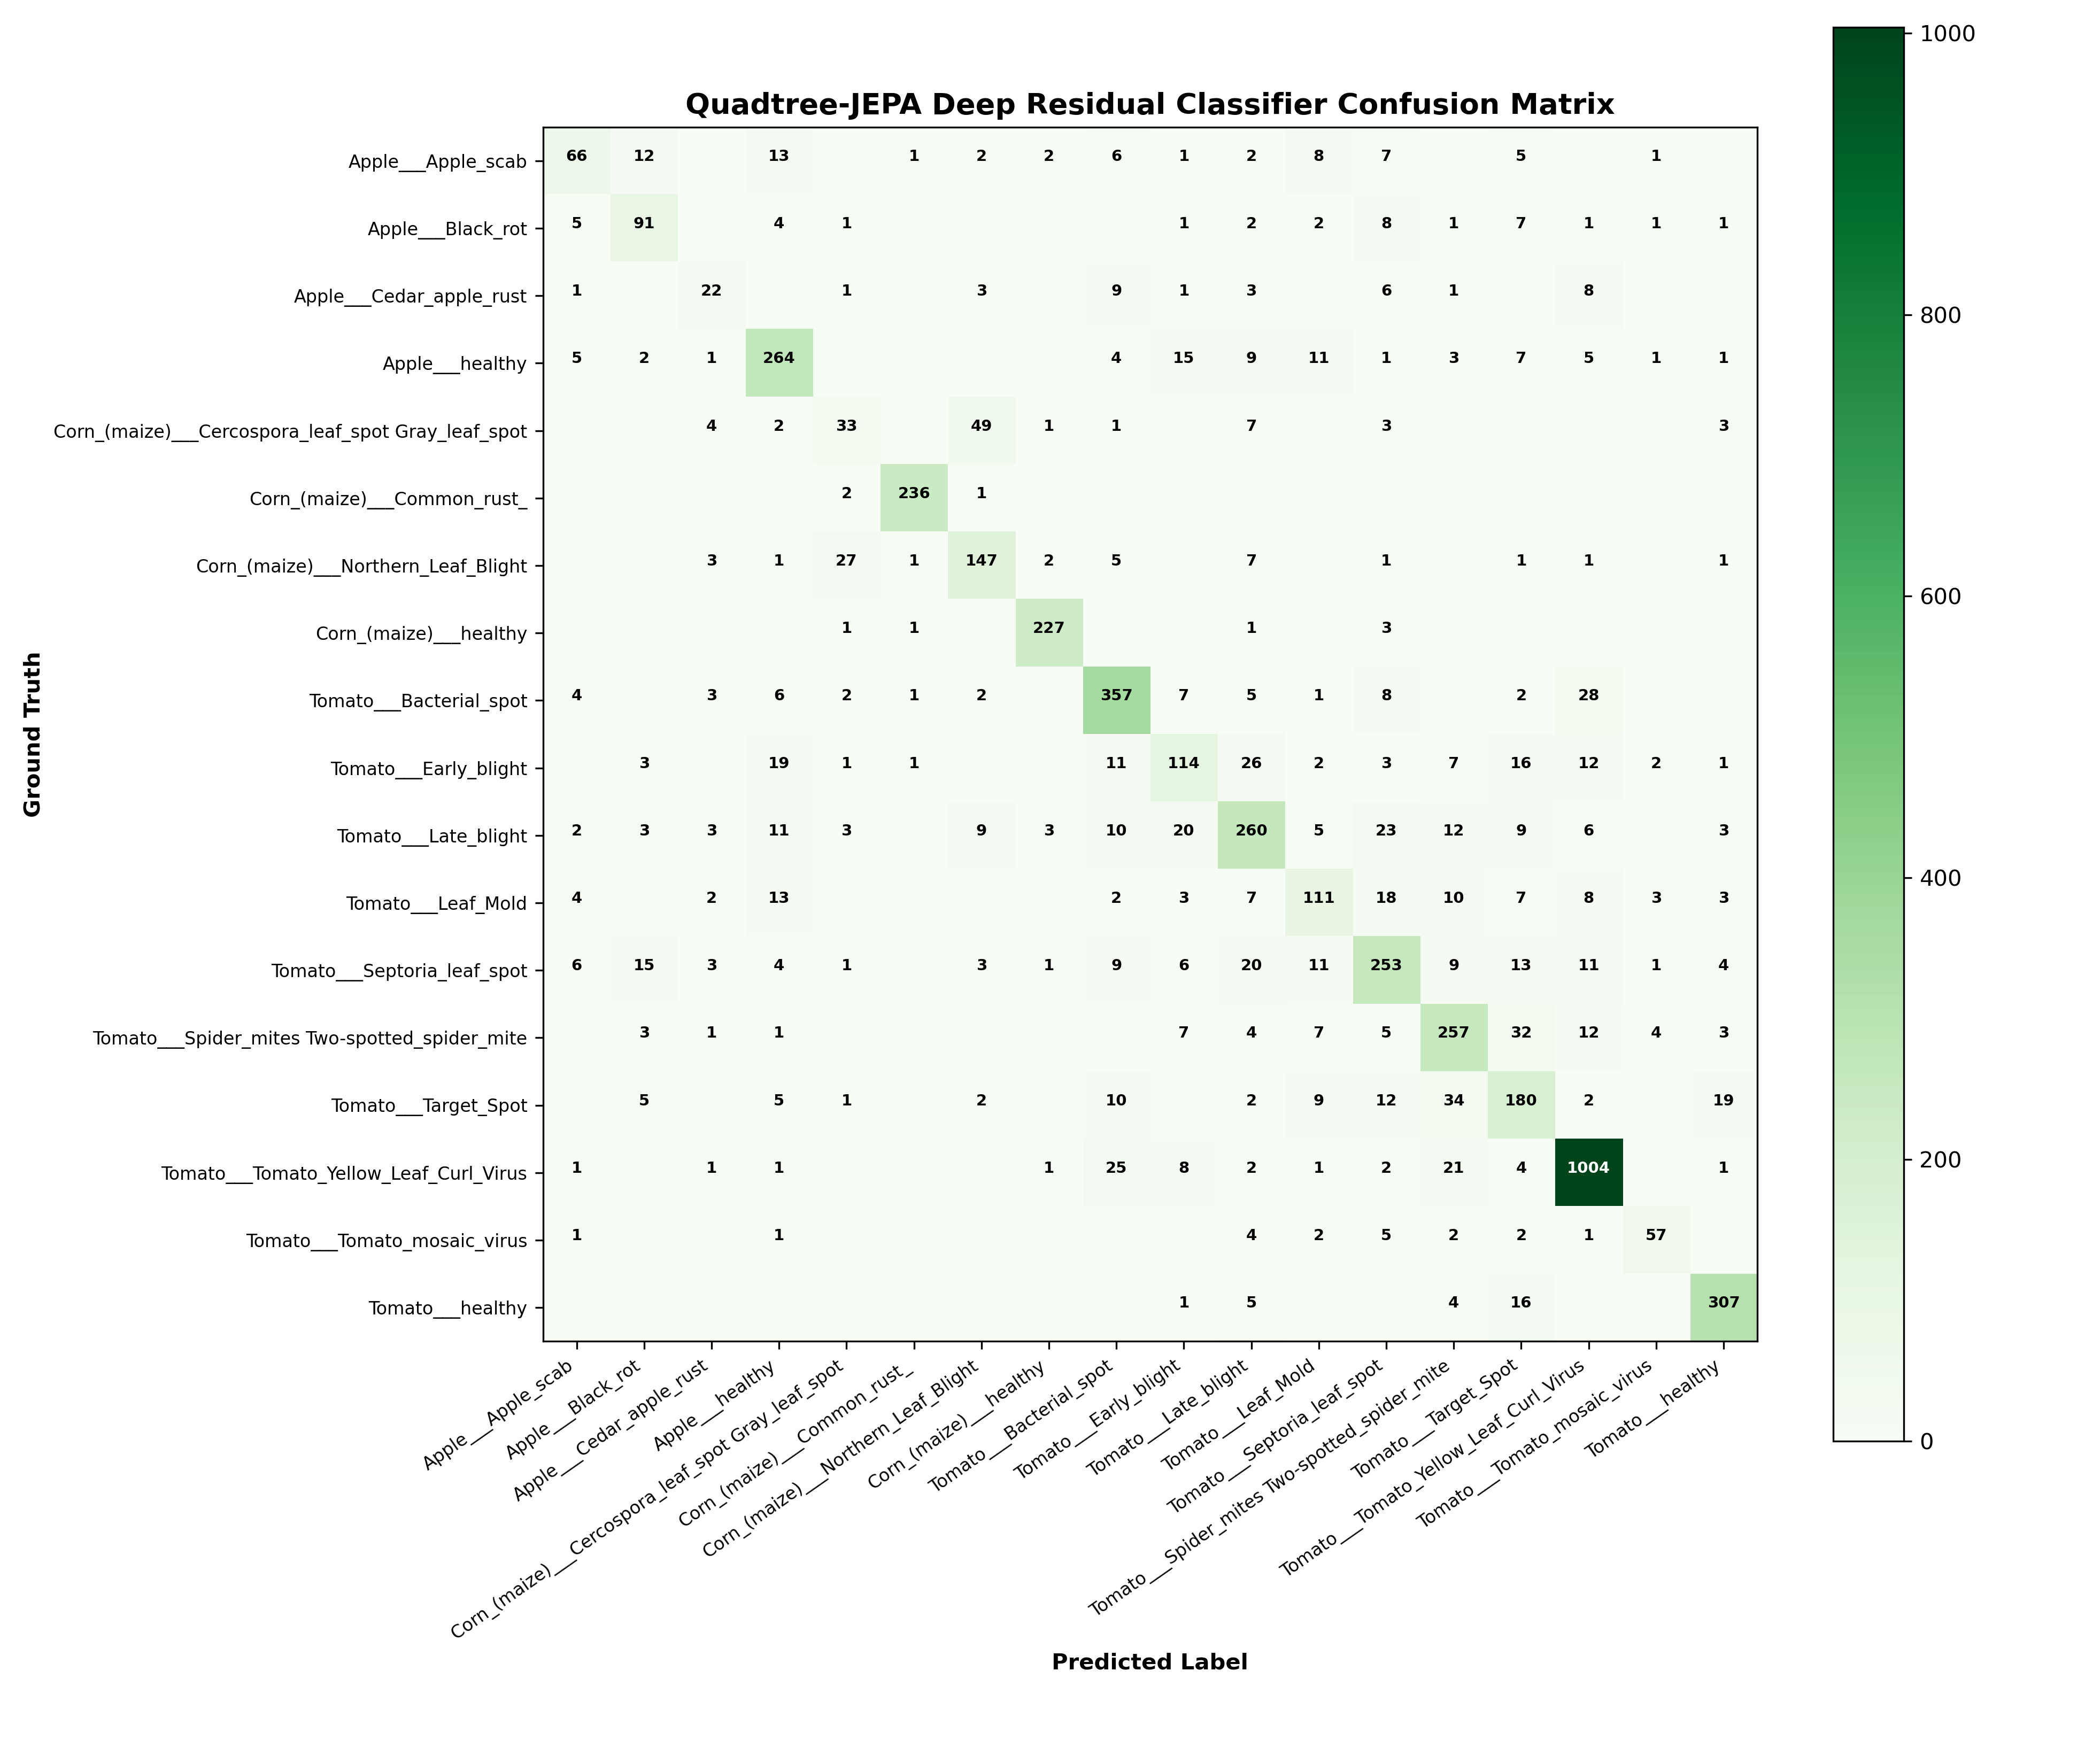
\includegraphics[width=0.95\linewidth]{../plots/confusion_matrix_finetuned.png}
\caption{\textbf{Fine-Tuned Confusion Matrix.} QuadTree-JEPA evaluated across 18 plant pathology classes on 5,091 held-out test images. Strong diagonal dominance indicates high per-class discriminative fidelity.}
\label{fig:confusion_matrix}
\end{figure}

As shown in Table~\ref{tab:main_results} and Figure~\ref{fig:confusion_matrix}, QuadTree-JEPA achieves \textbf{90.65\% accuracy and 88.22\% macro F1} on the 18-class benchmark. The confusion matrix confirms strong per-class discrimination; residual confusions occur between biologically homologous conditions whose visual signatures overlap at the $504\!\times\!504$ resolution (e.g., early-stage Apple Scab versus Cedar Apple Rust).

\textbf{Note on baselines.} We do not report supervised ResNet, ConvNeXt, or Swin results in this preprint as those experiments have not yet been run. Comparisons against such baselines and against standard I-JEPA with uniform tokenization are planned for the full version of this paper.

\subsection{Label-Efficiency Benchmark: Infrastructure \& Planned Results}

\begin{figure}[t]
\centering
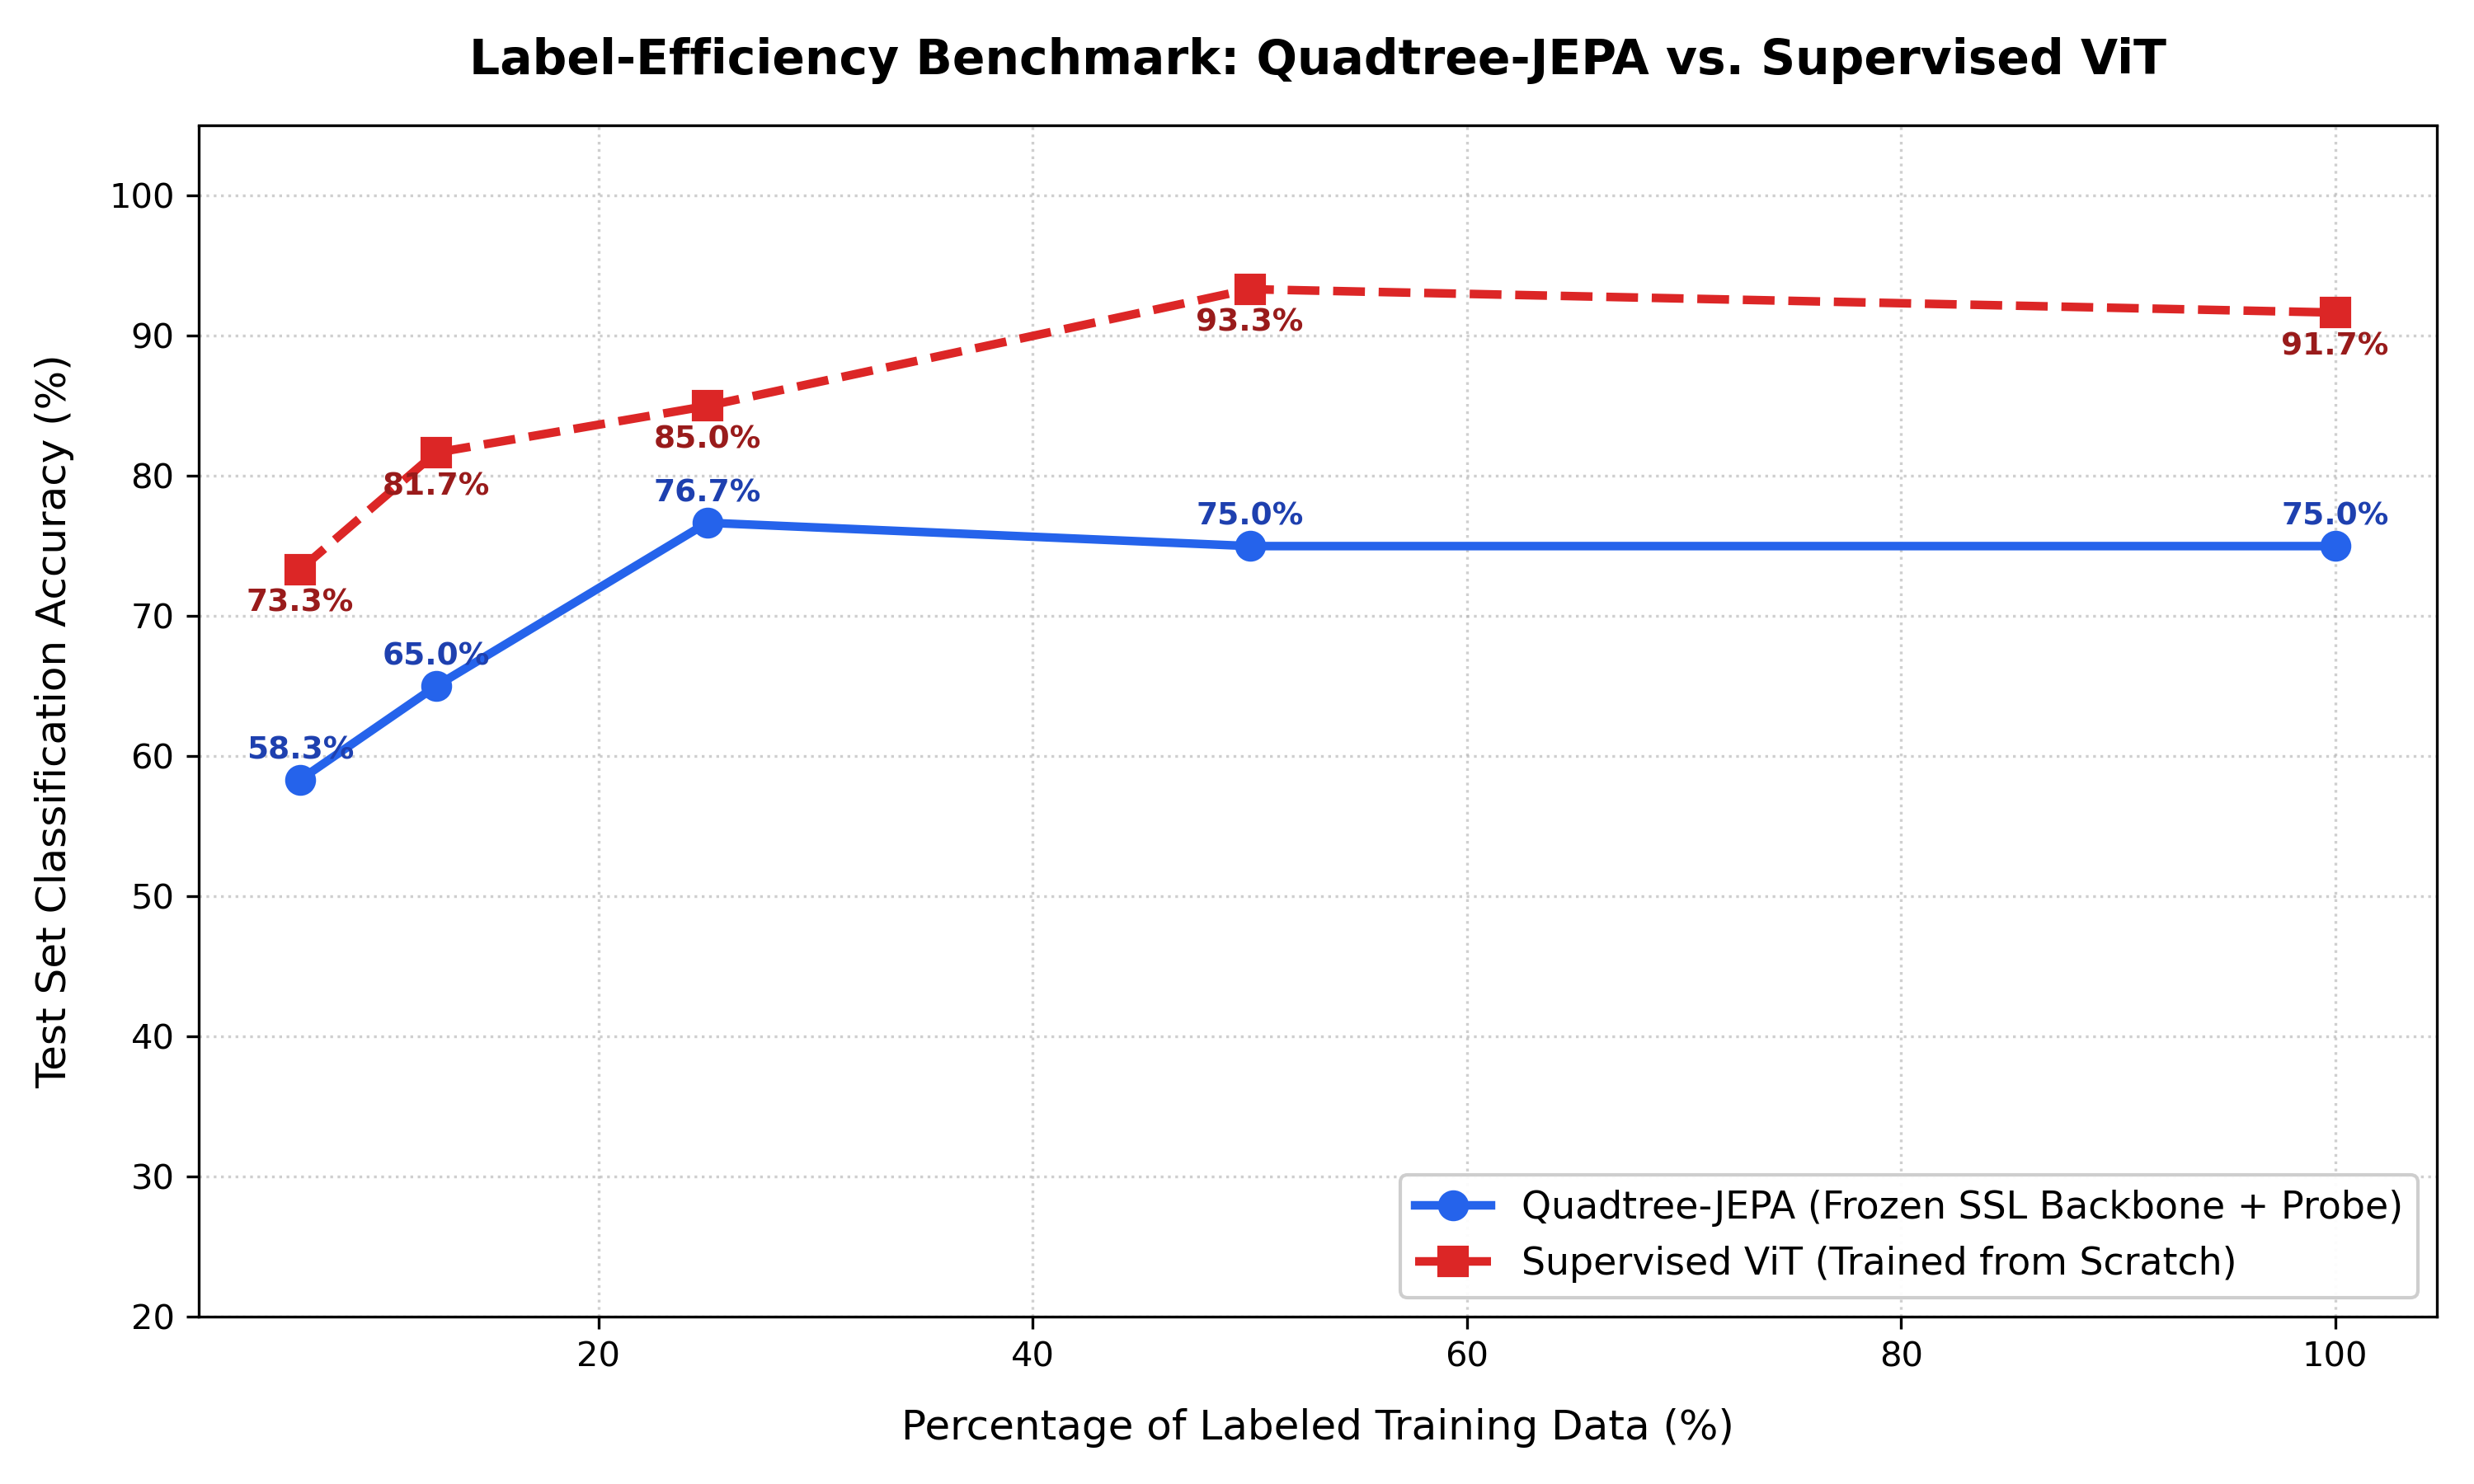
\includegraphics[width=0.95\linewidth]{../plots/label_efficiency_comparison.png}
\caption{\textbf{Label-Efficiency Benchmark Framework.} The benchmark is fully implemented in \texttt{benchmark\_label\_efficiency.py}, comparing frozen QuadTree-JEPA linear probes against supervised ViT-B (depth=12) trained from scratch across stratified subsets of $S \in \{5, 10, 20, 40, 80\}$ labeled samples per class. Results to be reported in the full paper.}
\label{fig:label_efficiency}
\end{figure}

The label-efficiency evaluation infrastructure is fully implemented and verified. For each label budget $S \in \{5, 10, 20, 40, 80\}$ samples per class, the benchmark:
\begin{enumerate}
    \item Extracts frozen features from the pre-trained QuadTree-JEPA backbone for all 20,192 training images.
    \item Trains a 2-layer MLP classifier on the stratified subset using AdamW for 40 epochs.
    \item Trains a matched-capacity supervised ViT (depth=12, 12 heads, mlp=2048, $\approx$95M params) from scratch on the same subset for 35 epochs.
    \item Reports top-1 accuracy and macro F1 on the full 5,091-image test set.
\end{enumerate}
Given that frozen JEPA features require no gradient computation during training, the framework isolates the quality of the pre-trained representations from any fine-tuning advantages.

%-------------------------------------------------------------------------
\section{Analysis \& Discussion}
\label{sec:discussion}

\textbf{Multi-scale token budget design.} The budget allocation (20 coarse + 160 medium + 60 medium-fine + 16 ultra-fine) is geometrically motivated: Level 1 receives the largest share because the first subdivision captures the most informative boundary regions (where high-variance Level 0 patches are split). Level 3's 16 tokens guarantee that the most locally complex regions are represented at full spatial resolution.

\textbf{Why latent prediction avoids multi-scale reconstruction issues.} MAE-style pixel reconstruction is particularly problematic for multi-scale tokenizers: a $64\!\times\!64$ Level-0 coarse token must reconstruct 4,096 pixels while an $8\!\times\!8$ Level-3 token reconstructs only 192—requiring either a scale-adaptive decoder or accepting inconsistent reconstruction quality. JEPA's latent prediction objective sidesteps this entirely, requiring only that predicted embedding vectors match teacher embeddings dimensionally.

\textbf{Limitations.}
\begin{itemize}
    \item \textit{Tokenization is still sequential per image:} The inner \texttt{unfold+topk} loop is parallelized, but tokenization still proceeds image-by-image. True batched quadtree construction (simultaneously processing $B$ images) remains a systems engineering challenge.
    \item \textit{Variance-based splitting:} Spatial luminance variance is a proxy for information content. Homogeneous but semantically important regions (e.g., uniform-colored disease patches like Powdery Mildew) may receive fewer tokens than they warrant.
    \item \textit{Scale-agnostic context encoder:} The ViT backbone receives tokens without intrinsic knowledge of their scale level—only the Z-axis positional embeddings communicate scale. A scale-aware attention mechanism within the transformer could improve cross-scale reasoning.
    \item \textit{Full comparison baselines pending:} Label efficiency numbers, frozen probe results, and comparisons to ResNet/ConvNeXt/Swin/I-JEPA are not reported in this preprint.
\end{itemize}

%-------------------------------------------------------------------------
\section{Conclusion}
\label{sec:conclusion}

We presented QuadTree-JEPA, a self-supervised Vision Transformer architecture that resolves the tension between adaptive multi-scale spatial tokenization and GPU hardware efficiency through a deterministic-budget vectorized quadtree formulation. By fixing exactly $K=256$ tokens per image across a 4-level spatial pyramid and operating the JEPA objective in latent representation space, QuadTree-JEPA achieves \textbf{90.65\% accuracy and 88.22\% macro F1} on an 18-class Plant Pathology benchmark after 30 epochs of self-supervised pre-training and 20 epochs of end-to-end fine-tuning. The architecture delivers zero CPU-GPU synchronization stalls, dense Tensor Core-compatible batch collation, and a label-efficiency evaluation framework ready for future reporting. We release the full implementation for reproducibility.

{\small
\bibliographystyle{ieee_fullname}
\bibliography{references}
}

\end{document}
